

% trial .tex file %
\documentclass[9pt]{article}  % specifies document class (article) and point size (10pt)
\usepackage{graphicx}
\usepackage{polski}
\usepackage[utf8]{inputenc}
\usepackage{sidecap}
\usepackage{wrapfig}
\usepackage{subfig}
\usepackage{amsmath}
\usepackage{float}
\usepackage{enumerate}
\usepackage{listings}
\usepackage{listings}
\usepackage{color}

\definecolor{dkgreen}{rgb}{0,0.6,0}
\definecolor{gray}{rgb}{0.5,0.5,0.5}
\definecolor{mauve}{rgb}{0.58,0,0.82}

\lstset{
  language=R,
  aboveskip=3mm,
  belowskip=3mm,
  showstringspaces=false,
  columns=flexible,
  basicstyle={\small\ttfamily},
  numbers=none,
  numberstyle=\tiny\color{gray},
  keywordstyle=\color{blue},
  commentstyle=\color{dkgreen},
  stringstyle=\color{mauve},
  breaklines=true,
  breakatwhitespace=true,
  tabsize=3
}


\begin{document}               % starts document
\author{Michał Kubica}
\title{Modele Liniowe \\ Raport nr 5}       
\maketitle                     % constructs big, fancy title

\section{Zadanie 1}            % makes a section header





  Dany jest model:
  $$Y = \beta_0 + \beta_1 X_1 + \beta_2 X_2 + \epsilon  $$
  oraz estymatory: $b_0 = 1, b_1 = 4, b_2 = 3, s=3$
  \subsection{a)}
  
  $pred\left(Y|X_1 = 2, X_2=6\right) = 1+4\cdot 2 + 3 \cdot 6 = 27$
  \subsection{b)}
  Wiemy, że
  $$s^2( \hat{\mu}_h ) = s^2 X'_h(X'X)^{-1}X_h = 2^2 = 4 $$
  Zatem,
  $$ s^2(pred) = s^2( 1+X'_h(X'X)^{-1}X_h ) = s^2 +s^2(X'_h(X'X)^{-1}X_h) = 3^2+4 = 13  $$
  
  
  \subsection{c)}
  
  Liczba obserwacji: $n=20$ oraz $s(b_1) = 1$ \newline
  95\% przedział ufności na poziomie istotności $\alpha=0.05$:
  $$b_1 \pm t_{n-1}^{-1} \left( 1-\frac{0.05}{2}\right) s(b_1)$$
  co daje:
  $$ 4 \pm 2.093024$$
  
\section{Zadanie 2}
  
  \begin{table}[H]
  \centering
    \begin{tabular}{c|cc}
     & Typ I & Typ II  \\ \hline
     $X_1$ & 300 & 30  \\ 
     $X_2$ & 40 & 25   \\ 
     $X_3$ & 20  & ? \\ 
  \end{tabular} 
  \end{table}

  Wiemy, że $SST = 760$ i liczba obserwacji $n= 24$


  \subsection{a)}
  Suma kwadratów typu II dla zmiennej $X_3$ to różnica sumy kwadratów w modelu pełnym i bez $X_3$:\newline
  $SS(X_1, X_2) - SS(X_1, X_2, X_3)  = SS(X_3 | X_1, X_2)$ \newline
  Zauważmy, że prawa strona równości odpowiada różnicy sumy kwadratów dla modelu z $X_3$ i bez $X_3$, zatem jest to suma kwadratów typu I dla zmiennej $X_3$. Stąd "?" w tabeli jest równy 30.
  
  
  \subsection{b)}
  Testujemy hipotezę:
  $$H_0: \beta_0 \ne 0, \beta_1 =0, \beta_2 \ne 0, \beta_3 \ne 0 $$
  $$H_A: \beta_0 \ne 0 \vee \beta_1 \ne 0 \vee \beta_2 \ne 0 \vee \beta_3 \ne 0$$
   Wiemy, że $$SSM(X_1, X_2, X_3) = SSM(X_1) + SSM(X_2 | X_1) + SSM(X_3 | X_1, X_2) = 300 + 40 + 20 = 360$$
   Zatem
   $$ SSE = SSE(X_1, X_2, X_3) = SST(X_1, X_2, X_3) - SSM(X_1, X_2, X_3) = 760 - 360 = 400 $$
  
  $$F = \frac{MSM}{MSE} = \frac{ \frac{SSM(X_1 | X_2, X_3)}{4-3}  }{ \frac{SSE}{24-4} } = 
  \frac{ \frac{30}{1}  }{ \frac{400}{20} } = 1,5$$
  
  Przy prawdziwości hipotezy zerowej $F \sim F(1,20)$. Przy poziomie istotności $\alpha = 0.05$ wartość krytyczna wynosi $4.351244$. Zatem nie odrzucamy hipotezy zerowej.
  
  
  \subsection{c)}
    Testujemy hipotezę:
  $$H_0: \beta_2= \beta_3 = 0$$
  $$H_A: \beta_2 \ne 0 \vee \beta_3 \ne 0 $$
  
  $$F = \frac{MSM}{MSE} = \frac{ \frac{SSM(X_2, X_3 | X_1)}{4-2}  }{ \frac{SSE}{24-4} } = \frac{ \frac{ SSM(X_1, X_2, X_3) - SSM(X_1) }{4-2}  }{ \frac{SSE}{24-4} } = \frac{ \frac{ 360-300 }{4-2}  }{ \frac{400}{24-4} } = \frac{3}{4}$$
    Przy prawdziwości hipotezy zerowej $F \sim F(2,20)$. Przy poziomie istotności $\alpha = 0.05$ wartość krytyczna wynosi $3.492828$. Zatem nie odrzucamy hipotezy zerowej.
  
  
  \subsection{d)}
  
  
      Testujemy hipotezę:
  $$H_0: \beta_1 = \beta_2= \beta_3 = 0$$
  $$H_A: \beta_1 \ne 0 \vee \beta_2 \ne 0 \vee \beta_3 \ne 0 $$
  
  $$F = \frac{MSM}{MSE} = \frac{ \frac{SSM(X_1, X_2, X_3)}{4-3}  }{ \frac{SSE}{24-4} } = \frac{ \frac{ 360 }{3}  }{ \frac{400}{20} } = 6$$
  
  
      Przy prawdziwości hipotezy zerowej $F \sim F(3,20)$. Przy poziomie istotności $\alpha = 0.05$ wartość krytyczna wynosi $3.098391$. Zatem odrzucamy hipoteze zerową.
  
  \subsection{e)}
  
  Dla modelu:
  $$Y = \beta_0 + \beta_1 X_1 + \epsilon$$
  Przetestowano hipotezę:
  $$H_0: \beta_1 = 0$$
  $$H_A: \beta_1 \ne 0$$
  
    $$F = \frac{MSM}{MSE} = \frac{ \frac{SSM}{dfM}  }{ \frac{SSE}{dfE} } = 
    \frac{ \frac{SSM(X_1)}{dfM}  }{ \frac{SST-SSM}{dfE} } = \frac{ \frac{300}{1}  }{ \frac{460}{22} } = 14.34783$$
  
        Przy prawdziwości hipotezy zerowej $F \sim F(1,22)$. Przy poziomie istotności $\alpha = 0.05$ wartość krytyczna wynosi $4.30095$. Zatem odrzucamy hipotezę zerową.
  
  
  \subsection{f)}
  
  $$R^2 = \frac{SSM}{SST} = \frac{300}{760} \approx 40\% $$
  
\section{Zadanie 3}



  \subsection{a)}
  Wygenerowano macierz $X_{100\times 2}$ taką, że wiersze są wektorami losowymi z rozkładu $N(0,\Sigma /100)$, gdzie 
  
  \[
  \Sigma = 
  \begin{bmatrix}
    1       & 0.9 \\
    0.9      & 1 \\
  \end{bmatrix}
  \]

  Następnie wygenerowano $Y = \beta_1 X_1 + \epsilon$, gdzie $\beta_1 = 3$ i $X_1$ jest pierwszą kolumną X. $\epsilon \sim N(0,1)$
  \subsection{b)}
  
  Dla dwóch modeli:
  \begin{equation}
  Y = \beta_0 + \beta_1 X_1 + \epsilon 
  \end{equation}
  
  \begin{equation}
  Y = \beta_0 + \beta_1 X_1 + \beta_1 X_2 + \epsilon 
  \end{equation}
  , gdzie $X_1$ i $X_2$ to dopowiednio, pierwsza i druga kolumna macierzy X.
  
  
  Dla obu modeli Wyznaczono 95\% przedział ufności dla $\beta_1$ i przetestowano hipotezę zerową o zerowaniu się $\beta_1$. Porównano wyniki z poniższej tabeli.
  
    \begin{table}[H]
  \centering
    \begin{tabular}{c|c|c}
     Model & przedział ufności & p-wartość \\
         \hline
     1 & (2.084178984, 6.4838348) & $0.0002$ \\
     2 & (-0.913786253, 9.0837873) & $0.1081 $ \\
  \end{tabular} 
  \end{table}
  
  W pierwszym modelu odrzucono hipotezę zerową o zerowaniu się $\beta_1$. W drugim modelu nie ma podstaw do odrzucenia hipotezy zerowej. Takie wyniki są spowodowane tym, że wektory $X_1$ i $X_2$ są bardzo mocno skorelowane, więc w drugim modelu Y może być objaśniony zarówno przez $X_1$ jak i $X_2$.
  
  \subsection{c)}
  
  Estytmator wariancji $\beta_1$ wyliczono ze wzoru:
  $$s(\beta_1) = \sqrt{ \frac{e'e}{n-p} (X'X)^{-1}  }$$
  , gdzie \newline
  $e = Y - \hat{Y} $ \newline
  $ X = (1, X_1)$ - dla pierwszego modelu \newline
  $ X = (1,X_1, X_2)$ - dla drugiego modelu \newline
  Następnie wiedząc, że przy prawdziwości hipotezy alternatywnej o niezerowaniu się współczynnikia $\beta_1$ statystka testowa F ma rozkład F-Snedecora z parametrem niecentralności $\delta = (\frac{\beta_1}{s(\beta_1)})^2$ obliczono moc identyfikacji $X_1$ jako 
  $$ moc = 1-(F^{-1}( F_{kryt}(0.95, p-1,n-p)  ,p-1, n-p ) )  $$ 
  Wyniki przedtsawiono w poniższej tabeli
  
    
  \begin{table}[H]
  \centering
    \begin{tabular}{c|c|c}
     Model & odchylenie standardowe $\beta_1$ & moc testu \\
         \hline
     1 & 1.010875 & 83.61\% \\
     2 & 2.199348 & 20.69\% \\
  \end{tabular} 
  \end{table}
  
  
  

  \subsection{d)}
  
  Wygenerowano 1000 kopii wektora błędów $\epsilon$ oraz odpowiadające im wektory zmiennej objaśnianej Y. Następnie 1000 razy wyestymowano estymator $\beta_1$. Obliczono odchylenie standardowe $\beta_1$ oraz zliczono procentowow ile razy nie został popełniony błąd I rodzaju. Wyniki przedstawiono w poniższej tabeli. 
  
  \begin{table}[H]
  \centering
    \begin{tabular}{c|c|c}
     Model & odchylenie standardowe $\beta_1$ & moc testu \\
         \hline
     1 & 0.9659516 & 86.86\% \\
     2 & 2.281101 & 24.4\% \\
  \end{tabular} 
  \end{table}


\section{Zadanie 4}

  \subsection{a)}
  
    Wyniki zadania przedstawiono w tabeli.
      \begin{table}[H]
  \centering
    \begin{tabular}{c|c|c|c|c|c|c}
     ilość zmiennych & SSE & MSE & AIC & p-wartość1 & p-wartość2 & fałszywe odkrycia \\ \hline
    2 & 27386.02 & 33.6892 & 6155.91 & 0 & 0  & 0 \\
    5 & 978.7171 & 3.884364 & 2830.364 & 0 & 0 & 0 \\
    10 & 967.7282 & 14.87326 & 2829.073 & 0 & 0 & 0 \\
    50 & 915.9179 & 66.6836 & 2854.048 & 0 & 0 & 5 \\
    100 & 847.1921 & 135.4094 & 2876.049 & 0 & 0 & 11 \\
    500 & 442.3119 & 540.2895 & 3026.137 & 0 & 0 & 39 \\
    950 & 40.07491 & 942.5266 & 1524.872 & 0 & 0 & 56 \\
  \end{tabular} 
  \end{table}
  Tylko na podstawie kryterium AIC wybrano model z 950 zmiennymi objaśniającymi.
  
  \subsection{b)}
  
  Wyniki zadania przedstawiono w tabeli.
        \begin{table}[H]
  \centering
    \begin{tabular}{c|c|c|c|c|c|c}
     ilość zmiennych & SSE & MSE & AIC & p-wartość1 & p-wartość2 & fałszywe odkrycia \\ \hline
    2 & 28711.03 & 173.8838 & 6203.158 & 0 & 0  & 0 \\
    5 & 1017.685 & 3.623658 & 2869.407 & 0 & 0 & 0 \\
    10 & 944.5689 & 5.289108 & 2804.85 & 0 & 0 & 0 \\
    50 & 1043.206 & 54.02967 & 2984.176 & 0 & 0 & 2 \\
    100 & 933.7523 & 92.12432 & 2973.333 & 0 & 0 & 5 \\
    500 & 463.4319 & 478.5233 & 3072.781 & 0 & 0 & 23 \\
    950 & 48.07952 & 929.0837 & 1706.978 & 0 & 0 & 22 \\
  \end{tabular} 
  \end{table}
  
  Tylko na podstawie kryterium AIC wybrano model z 950 zmiennymi objaśniającymi.


\section{Zadanie 5}

Dopasowany model regresji:
$$ Y_{satisfaction} = 1.053245-0.005861 X_{age} + 0.001928 X_{severity} + 0.030148 X_{anxiety}$$

Przetestowano hipotezę:
$$H_0: \beta_1 = \beta_2 = \beta_3 = 0$$
$$H_A: \beta_1 \ne 0 \vee \beta_2 \ne 0 \vee \beta_3 \ne 0$$

  \begin{table}[H]
  \centering
    \begin{tabular}{|c|c|c|c|c|c|}
    \hline
     $R^2$ & statystyka F & $df_{licznika}$ & $df_{mianownika}$ & p-wartość \\
    \hline
    0.5088 & 16.54 & 3 & 42 & $3.043 \cdot 10^{-7}$ \\
    \hline
  \end{tabular} 
  \end{table}


\indent Ze względu na bardzo małą p-wartość odrzucamy hipotezę zerową. Jednak mała wartość współczynnika determinacji wskazuje na słabe dopasowanie modelu do danych.  


\section{Zadanie 6}

Model:
$$ Y_{satisfaction} = \beta_0 + \beta_1 X $$

Kolejno dla zmiennych objaśniających (age, severity, anxiety) przetestowano hipotezę:
$$H_0: \beta_1 = 0$$
$$H_A: \beta_1 \ne 0$$

  \begin{table}[H]
  \centering
    \begin{tabular}{c|c|c|c|c|c|}
     X & $R^2$ & statystyka & $df$ & p-wartość & przedział ufności dla $\beta_1$ \\ \hline
    Age & 0.4002 & -5.593  & 44  & $1.33 \cdot 10^{-6}$ & $(-0.01522837,-0.007160361)$ \\
    Severity & 0.3092 & 4.598  & 44  & $3.59 \cdot 10^{-5}$ & $(0.01073994,0.02750293)$\\
    Anxiety & 0.4496 & 0.4496  & 44  & $3.429 \cdot 10^{-7}$ & $(0.03088933,0.06217329)$\\
  \end{tabular} 
  \end{table}
  
  W każdym przypadku odrzucamy hipotezę zerową. Możemy patrzeć na p-wartość albo na to, że 0 nie należy do wyznaczonego przedziału ufności.




\section{Zadanie 7}

    \begin{figure}[H]
      \centering
      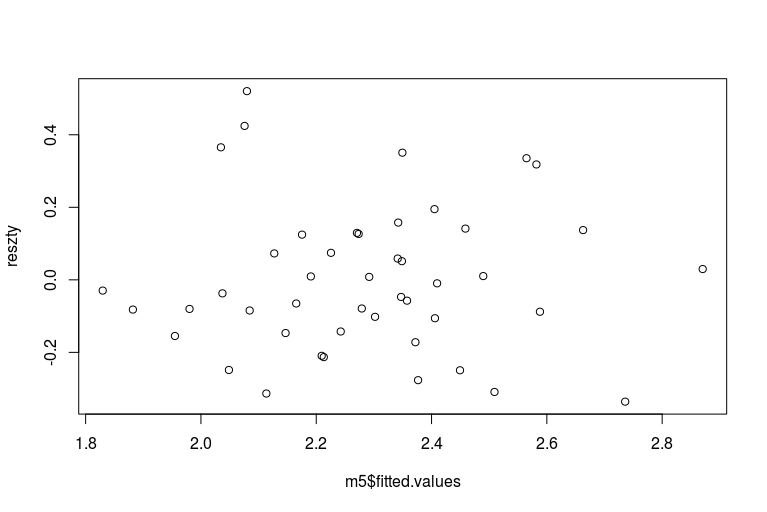
\includegraphics[width=0.7\textwidth]{71.png}
      \caption {}
    \end{figure} 
    \begin{figure}[H]
      \centering
      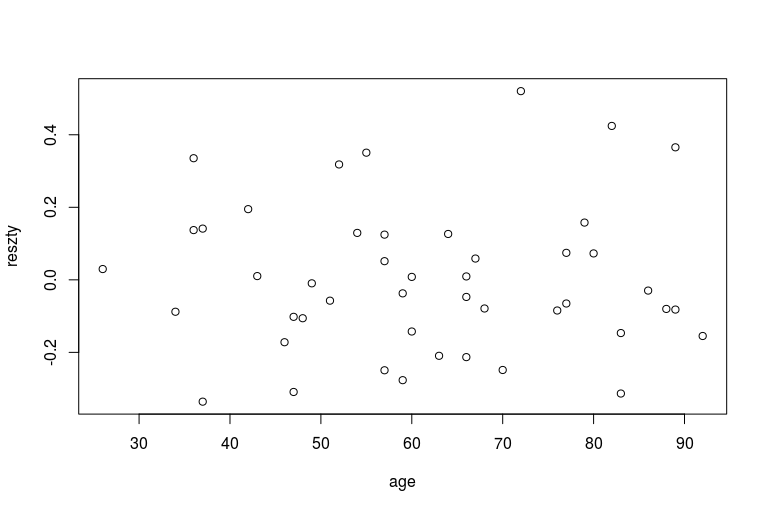
\includegraphics[width=0.7\textwidth]{72.png}
      \caption {}
    \end{figure} 
    \begin{figure}[H]
      \centering
      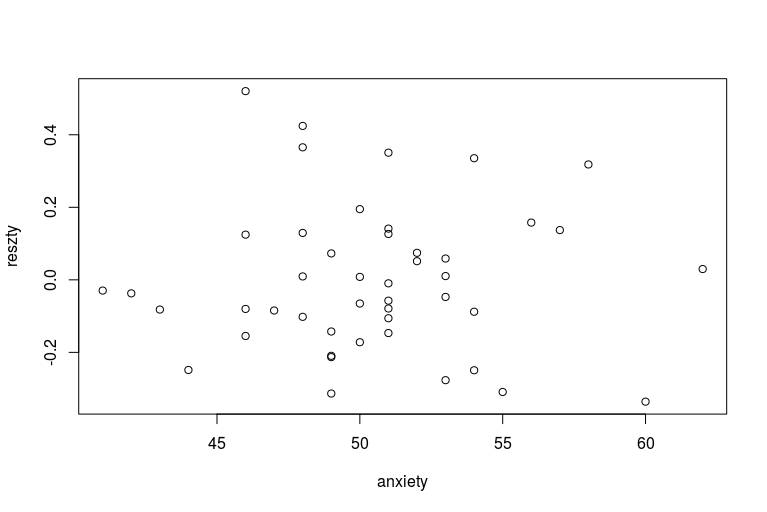
\includegraphics[width=0.7\textwidth]{73.png}
      \caption {}
    \end{figure} 
    \begin{figure}[H]
      \centering
      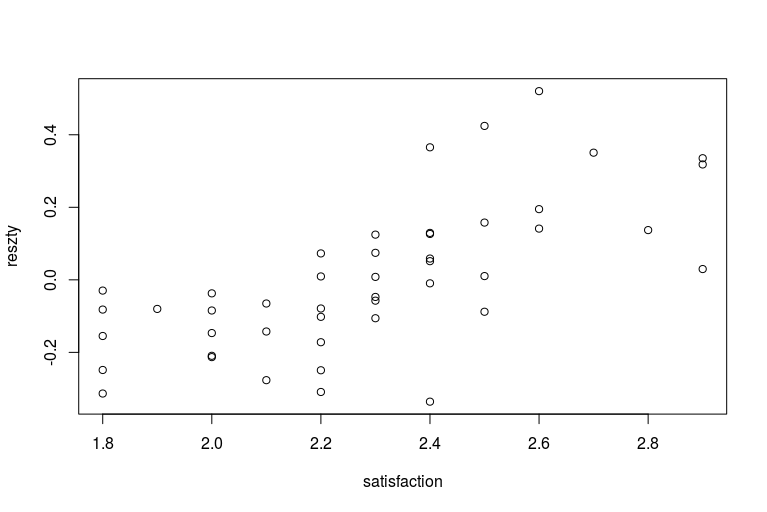
\includegraphics[width=0.7\textwidth]{74.png}
      \caption {}
    \end{figure} 
    
    Na wykresach widać sześć obserwacji, które mogą okazać się obserwacjami odstającymi, ze względu na to, że dane na osi X nie są posortowane względem występowania, obserwacje pojawiają się w różnych miejscach. Chmura punktów jest rozrzucona losowo, nie widać żadnej zależności pomiędzy zmiennymi na resztami.

\section{Zadanie 8}

    \begin{figure}[H]
      \centering
      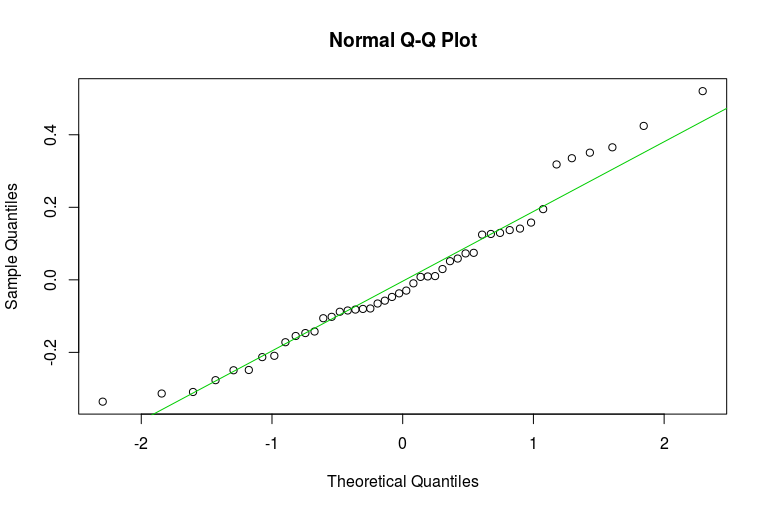
\includegraphics[width=0.7\textwidth]{8.png}
      \caption {Wykres kwantyl-kwantyl}
    \end{figure} 
    
\indent P-wartość dla testu Shapiro-Wilka wynosi $0.1481$. Zatem na poziomie istotności $\alpha=0.05$ nie ma podstaw do odrzucenia hipotezy zerowej o pochodzeniu reszt z rozkładu normalnego. Podobne wnioski wyciągnięto na podstawie wykresu kwantyl-kwantyl. Widać na nim, że rozkład reszt jest prawoskośny i ma cięższy prawy ogon, jednak zdecydowana większość punktów leży blisko prostej. Co świadczy o tym, że rozkład reszt jest zbliżony do $N(0,1)$.

\section{Zadanie 9}
\subsection{a)}

Utworzono w R dwa modele liniowe:
\begin{enumerate}[i)]
\item GPA $\sim$ HSM+HSS+HSE - model zredukowany(R)
\item GPA $\sim$ SATM+SATV+HSM+HSS+HSE - model pełny(F)
\end{enumerate}

Następnie licząc odpowiednie sumy kwadratów i stopnie swobody w modelu pełnym i zredukowanym obliczono wartość statystyki F przy testowaniu hipotezy zerowej o zerowaniu się współcyznników przy zmiennych objaśniających SATM i SATV.

$$ F = \frac{ \frac{SSE(R) - SSE(F)}{df(R) - df(F) } }{MSE(F) }  = 0.9503276$$
\subsection{b)}

    \begin{figure}[H]
      \centering
      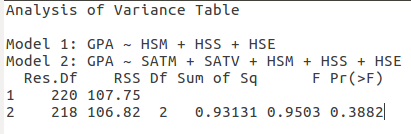
\includegraphics[width=0.7\textwidth]{9b.png}
      \caption {Analiza wariancji dla modelu pełnego i zredukowanego}
    \end{figure} 

  Z powyższej analizy wariancji dla obu modeli odczytujemy, że wartość statystyki F jest taka sama jak w otrzymana podpunkcie a). A p-wartość wynosi 0.3882, zatem nie ma podstaw do odrzucenia hipotezy zerowej o zerowaniu się współczynników przy zmiennych objaśniających SATM i SATV.

\section{Zadanie 10}

  \begin{table}[H]
  \centering
    \begin{tabular}{c|c|c}
     & Typ I & Typ II  \\ \hline
     SATM & 8.583 & 0.928  \\ \hline
     SATV & 0.001 & 0.233   \\ \hline
     HSM & 17.726  & 6.772 \\ \hline
     HSE & 1.891  &  0.957  \\ \hline
     HSS & 0.442 &  0.441  \\ 
  \end{tabular} 
  \end{table}

  \subsection{a)}
  Utworzono w R dwa modele liniowe:
  \begin{enumerate}[i)]
  \item GPA $\sim$ SATM+SATV+HSM - model 1
  \item GPA $\sim$ SATM+SATV - model 2
  \end{enumerate}
  
  A następnie obliczono sumy kwadratów w odpowiednich modelach ze wzorów: \newline
  $SSM_1 = \sum{(\hat{Y}_{i,1} - \bar{Y})^2 }$ \newline
  $SSM_2 = \sum{(\hat{Y}_{i,2} - \bar{Y})^2 }$ \newline
  $$SS(HSM | SATM, SATV) = SSM_1 - SSM_2 = \dots = 17.72647 $$
  Otrzymana wartość jest równa wartości w tabeli (typ I) dla zmiennej HSM.
  
  \subsection{b)}
  Dla zmiennej HSS odpowiadające jej sumy kwadratów odpowiednich typów to:
    \begin{enumerate}[1)]
  \item dla typu I - $SS(HSS | SATM,SATV,HSM,HSE)$ - model przed dodaniem HSS i po dodaniu HSS
  \item dla typu II - $SS(HSS | SATM,SATV,HSM,HSE)$ - model pełny i model bez HSS
  \end{enumerate}
  Zatem wartości tych sum będą takie same.


\section{Zadanie 11}
  Utworzono nową zmienną SAT, która jest zdefiniowana jako suma SATV i SATM. Utworzono w R model regresji GPA $\sim$ SATM+SATV+SAT, a następnie wywołano funkcję \textit{summary}.

    \begin{figure}[H]
      \centering
      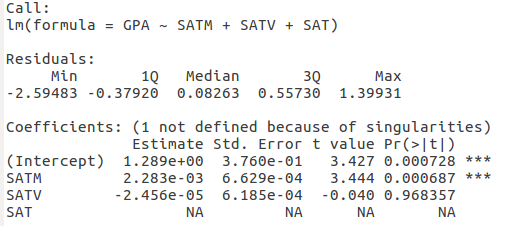
\includegraphics[width=0.7\textwidth]{11.png}
      \caption {}
    \end{figure} 

  Jak widać R sam zauważył, że macierz (XX') jest osobliwa, ponieważ SAT jest kombinacją liniową SATM i SATV. Z tego powodu nie wyestymował współczynnika przy zmiennej SAT (NA - Not Assigned).
  


\section{Zadanie 12}

    \begin{figure}[H]
      \centering
      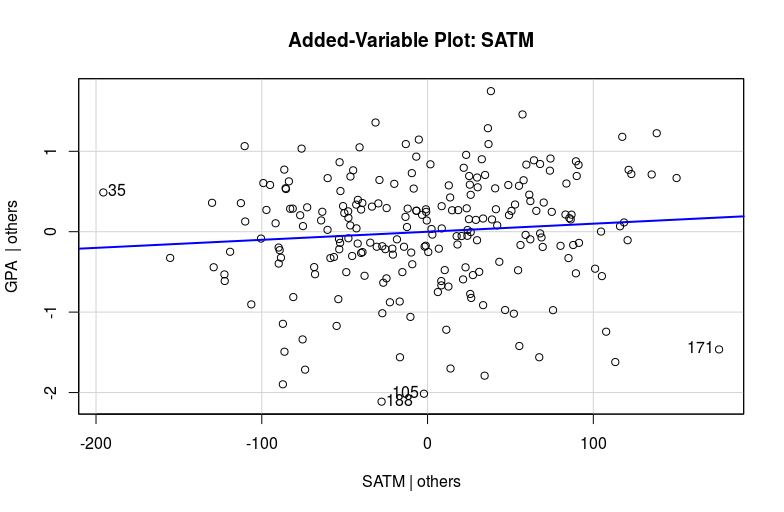
\includegraphics[width=0.9\textwidth]{121.png}
      \caption{Wykres częsciowej regresji dla SATM}
    \end{figure} 


    \begin{figure}[H]
      \centering
      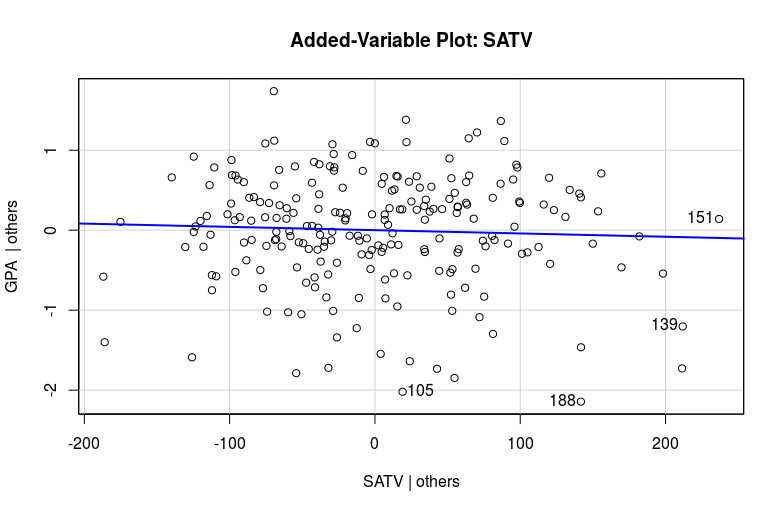
\includegraphics[width=0.9\textwidth]{122.png}
      \caption{Wykres częsciowej regresji dla SATV}
    \end{figure}
    
    
    \begin{figure}[H]
      \centering
      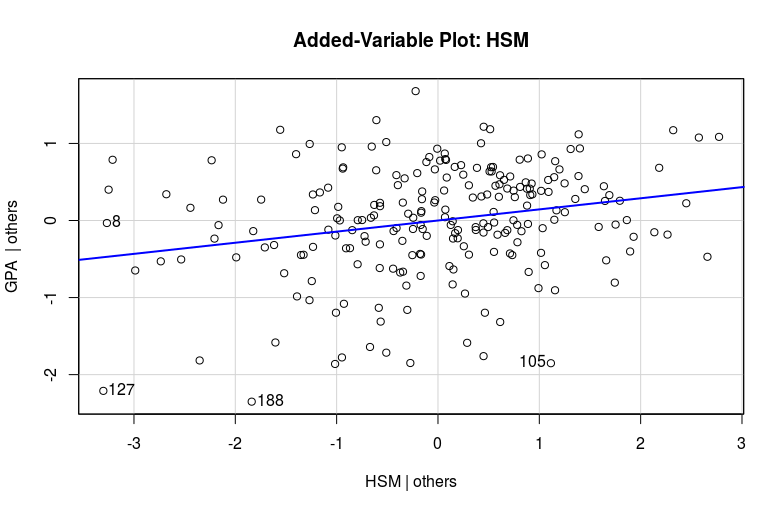
\includegraphics[width=0.9\textwidth]{123.png}
      \caption{Wykres częsciowej regresji dla HSM}
    \end{figure}


    \begin{figure}[H]
      \centering
      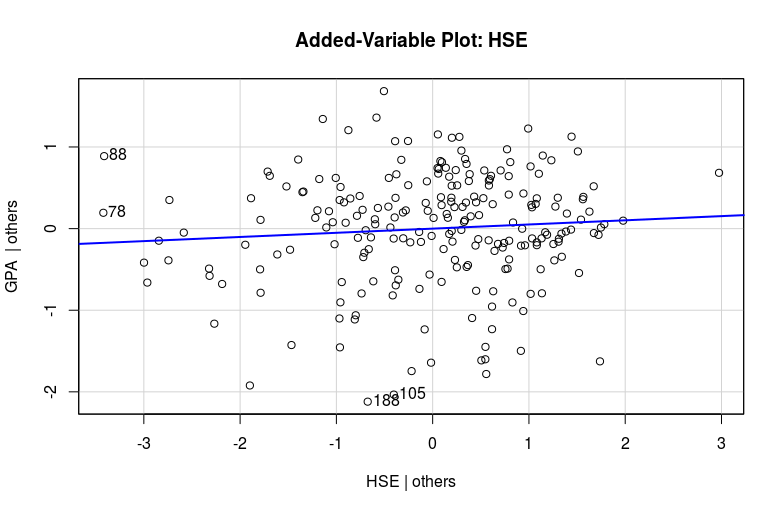
\includegraphics[width=0.9\textwidth]{124.png}
      \caption{Wykres częsciowej regresji dla HSE}
    \end{figure}
    
    
    \begin{figure}[H]
      \centering
      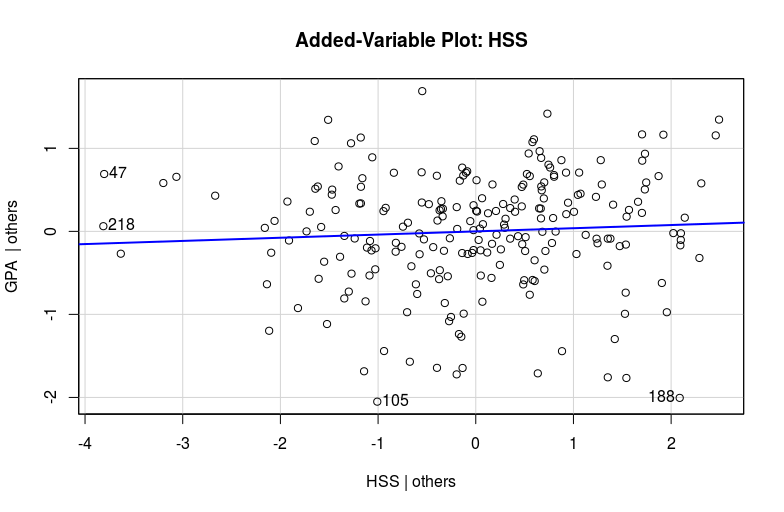
\includegraphics[width=0.9\textwidth]{125.png}
      \caption{Wykres częsciowej regresji dla HSS}
    \end{figure}
    
    
    \begin{figure}[H]
      \centering
      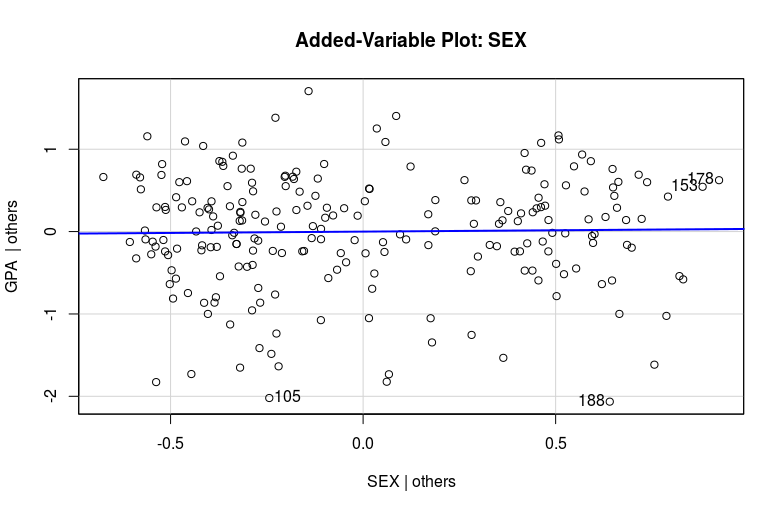
\includegraphics[width=0.9\textwidth]{126.png}
      \caption{Wykres częsciowej regresji dla SEX}
    \end{figure}

Wykresy częściowej regresji służą do badania obserwacji odstających i wpływowych. Na wykresach są zaznaczone numery obserwacji, które możemy uznać za wpływowe lub odstające. Są to bardzo przydatne typy wykresów pozwalające badać naturę pomiędzy zmienną objaśniającą a objaśnianą.


\section{Zadanie 13}

Obliczanie studentyzowanych reszt dla każdej obserwacji służy do identyfikowania obserwacji odstających, tak zwanych "outlierów". Studentyzowana reszta jest obliczana poniższym wzorem:

$$r_i = \frac{e_i}{ \sqrt{MSE(1-h_{ii})} }$$

Obserwacje uznaje się za odstającą jeżeli wartość bezwzgędna $r_i$ przekracza 3. W rozpatrywanym modelu zaobserwowano jedną obserwację odstającą (nr 188), którą również widać na poniższym wykresie.

    \begin{figure}[H]
      \centering
      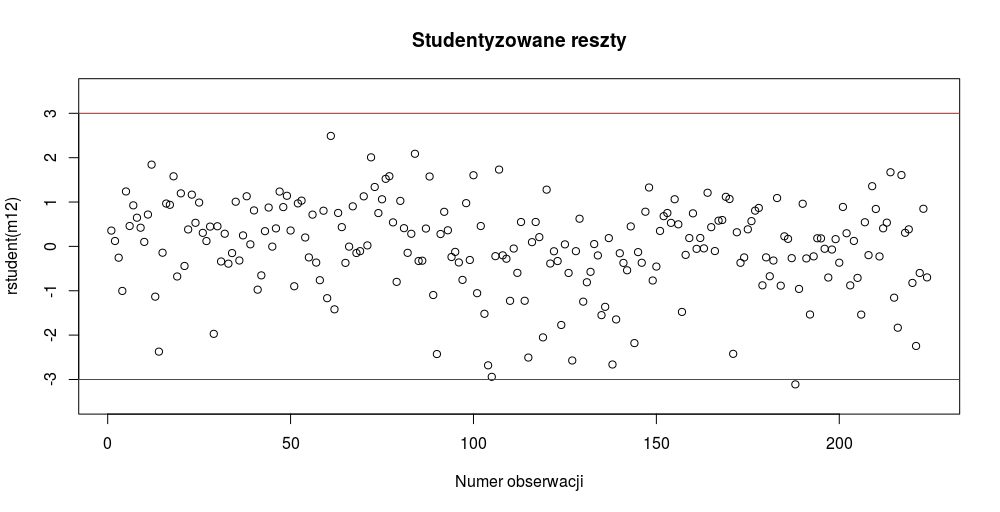
\includegraphics[width=0.9\textwidth]{13.png}
      \caption{Wykres studentyzowanych reszt}
    \end{figure} 



\section{Zadanie 14}

DFFITS jest narzędziem służącym do oceny czy dana obserwacja jest wpływowa. Inaczej, jest to miara wpływu danej obserwacji na model regresji. W praktyce usuwa się itą obserwację i porównuje się model pierwotny oraz model bez itej obserwacji. Odległość (miara) dana jest wzorem:

 $$ DFFITS_i = \frac{ \hat{y}_i - \hat{y}_{(i)} }{  \sqrt{MSE_{(i)} h_{ii}  } } $$

Dla małej liczby obserwacji przyjmuje się, ze obserwacja jest wpłyowa, jeżeli jej wartość bezwzględna z odległości DFFITS jest większa od 1. Dla dużej ilości obserwacji oblicza się wartość krytyczną powyżej, której obserwację uznaje się za wpływową. Jest wiele kryteriów według których wylicza się wartość krytyczną. W tym raporcie podaję dwa z nich:
$$  DFFITS_{kryt_1 } = 2\sqrt{ \frac{n}{p} } $$
$$  DFFITS_{kryt_2 } = 2\sqrt{ \frac{p+1}{n-p-1} } $$

Dla rozważanego modelu:
$$  DFFITS_{kryt_1 } = 0.3535534 $$
$$  DFFITS_{kryt_2 } = 0.3849002 $$


  
    \begin{table}[H]
  \centering
  \begin{tabular}{c|c}
     Numer obserwacji &  $DFFITS_{kryt_1 }$ \\ \hline
 12 & 0.4396709 \\
  29 & -0.3582333   \\
   84& 0.5759329   \\
   88& 0.4341960  \\
   90& -0.5522947  \\
   104& -0.4835059  \\
   107&  0.4183248  \\
   115& -0.3974564  \\
   119& -0.3681960  \\
   127& -0.6014848  \\
   138& -0.5020548  \\
   139& -0.4077397 \\
     
     
  \end{tabular} 
  \caption{Obserwowacje zakwalifikowane jako wpływowe wg pierwszego kryterium}
  \end{table}

  \begin{table}[H]
  \centering
  \begin{tabular}{c|c}
     Numer obserwacji &  $DFFITS_{kryt_2 }$ \\ \hline
     12 & 0.4396709 \\
     29& -0.3582333  \\
     84& 0.5759329  \\
     88& 0.4341960 \\
     90& -0.5522947 \\
     104& -0.4835059  \\
     107& 0.4183248 \\
     115& -0.3974564 \\
     119& -0.3681960 \\
     127& -0.6014848 \\
     138& -0.5020548 \\
     139& -0.4077397 \\
     144& -0.5062870 \\
     171& -0.5384145  \\
     183& 0.3542393 \\
     188& -0.7119046 \\
  \end{tabular} 
  \caption{Obserwowacje zakwalifikowane jako wpływowe wg drugiego kryterium}
  \end{table}
  

    \begin{figure}[H]
      \centering
      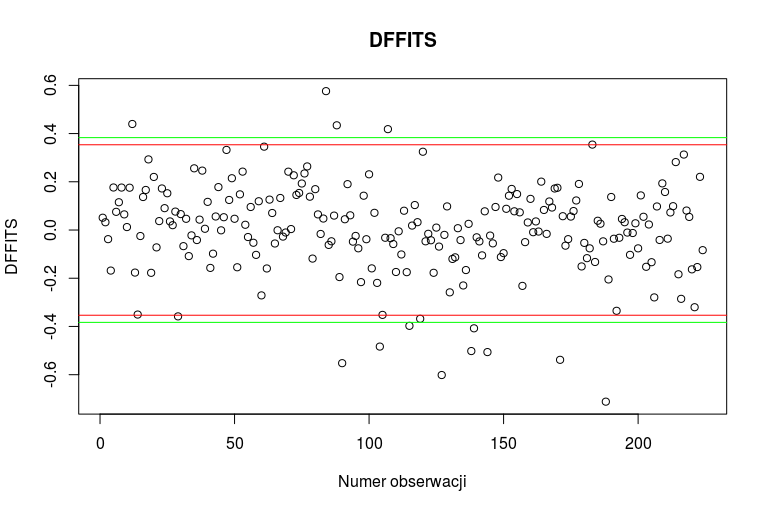
\includegraphics[width=0.7\textwidth]{14.png}
      \caption{Wykres DFFITS i wartości krytycznych (zielona i czerwona prosta)}
    \end{figure} 

Z tabel i wykresu możemy zidentyfikować obserwacje wpływowe.



\section{Zadanie 15}

Tolerancja jest to narzędzie diagnostyczne do sprawdzania, czy zmienne objaśniające da się przedstawić w przybliżeniu jako kombinację liniową innych zmiennych objaśniających. W ten sposób możemy decydować czy zmienną należy w modelu zostawić czy przyjrzeć jej się i ewentualnie pozbyć z modelu. Tolerancja jest definiowama jako 
$$tol = \frac{1}{VIF}$$
, gdzie VIF oznacza Variance Inflation Factor. \newline


  \begin{table}[H]
  \centering
  
    \begin{tabular}{c|c|c|c|c|c}
     SATM   &   SATV    &   HSM    &   HSE   &    HSS   &    SEX   \\ \hline
     0.5745498 & 0.7310535 & 0.5188628 & 0.5429546 & 0.5088203 & 0.7742519 
  \end{tabular} 
  \caption{Toleracja rozważanego modelu}
  \end{table}
  
  Przyjmuje się, że wartość tolerancji poniżej $0.1$ oznacza, że zmiennej należy się przyjrzeć pod kątem liniowej zależność od innych zmiennych. 

\section{Zadanie 16}
  Wywołując w R funkcję \textit{step} (dwustronnie) wybrano modele o najmniejszej wartości BIC lub AIC. W przypadku kryterium AIC był to model GPA $\sim$ HSM + HSE. W przypadku kryterium BIC - GPA $\sim$ HSM.

    \begin{figure}[H]
      \centering
      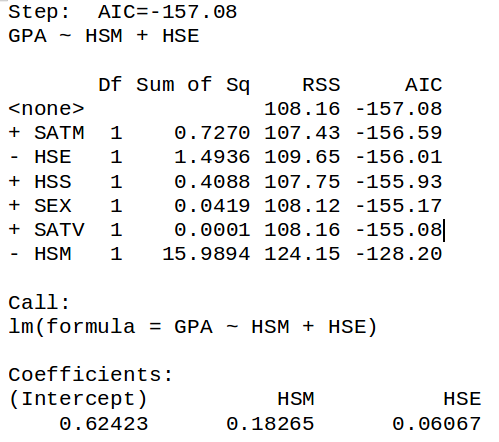
\includegraphics[width=0.7\textwidth]{161.png}
      \caption{AIC}
    \end{figure} 

    \begin{figure}[H]
      \centering
      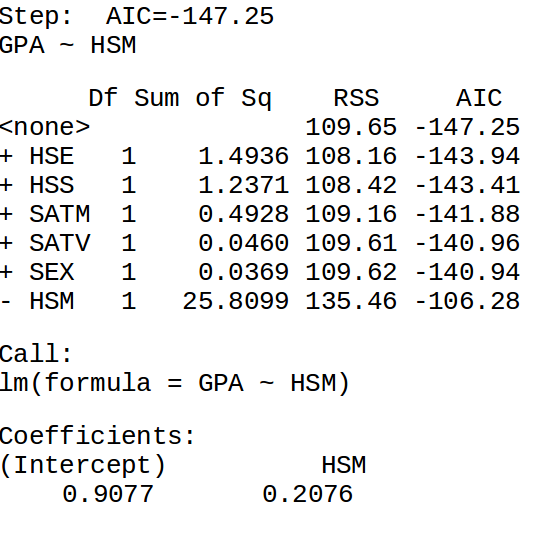
\includegraphics[width=0.7\textwidth]{162.png}
      \caption{BIC}
    \end{figure} 

  \section{Kod w R}
  
      \begin{lstlisting}




### ZAD 3 ###
# a)
library(mvtnorm)
sigma = matrix(c(1,0.9,0.9,1), 2,2)
X = rmvnorm(100,c(0,0),sigma/100)
X1 = X[,1]
X2 = X[,2]
eps = rnorm(100,0,1)
beta1 = 3
Y = beta1*X1+eps



# b)
m31 = lm(Y~X1)
e31=residuals(m31)
confint(m31)
summary(m31)$coefficients[2,1]

m32 = lm(Y~X1+X2)
e32=residuals(m31)
confint(m32)
summary(m32)
# c)
Y = cbind(rep(1,100), X1) %*% matrix(c(0,beta1),2,1)  + eps
Xprim = cbind(rep(1,100),X1)
H = Xprim %*% solve(matrix(t(Xprim) %*% Xprim ,2,2)) %*% t(Xprim)
sum(diag(H))
e = Y - H %*% Y
s1 = (t(e) %*% e) / ((100-2) * solve(matrix(t(Xprim) %*% Xprim ,2,2))[2,2])


Y = beta1*X1+eps
Xprim = cbind(rep(1,100), X1, X2)
H = Xprim %*% solve(matrix(t(Xprim) %*% Xprim ,3,3)) %*% t(Xprim)
sum(diag(H))
e = Y - H %*% Y
s2 = (t(e) %*% e) / (100-3) * solve(matrix(t(Xprim) %*% Xprim ,3,3))[2,2]

sqrt(s1)
sqrt(s2)
1-pf(qf(.95, 1, 98) , 1, 98, ncp=(3/sqrt(s1))^2)
1-pf(qf(.95, 2, 97) , 2, 97, ncp=(3/sqrt(s2))^2)


# d)
N=5000
p1 = rep(0,N)
p2 = rep(0,N)
beta11 = rep(0,N)
beta12 = rep(0,N)
for(i in 1:N){
  eps = rnorm(100,0,1)
  Y = beta1*X1+eps
  m10001 = lm(Y~X1)
  m10002 = lm(Y~X1+X2)
  beta11[i] = summary(m10001)$coefficients[2,1]
  beta12[i] = summary(m10002)$coefficients[2,1]
  
  p1[i] = summary(m10001)$coefficients[2,4]
  p2[i] = summary(m10002)$coefficients[2,4]
  
}
sd(beta11)
sd(beta12)
length(p1[p1<0.05]) / N * 100 #w procentach
length(p2[p2<0.05]) / N * 100 # w procentach

### ZAD 4 ###


X = matrix(rnorm(1000*950,0,1),1000,950)
eps = rnorm(1000)
beta = c(rep(3,5), rep(0,945))
Y = X %*% beta+eps

k=2
k
#a = summary(m10)$coefficients[1:k+1,1]
#a[order(a, decreasing=TRUE)[1:k]]
m10 = lm(Y~X[, order(a, decreasing=TRUE)[1:k]])


m10 = lm(Y~X[,1:k])
# suma reszta
sum((summary(m10)$residuals)^2)
# 
#anova(m10)[[2]][2]

# mean square error
sum((cbind(rep(1,1000),X[,1:k]) %*% m10$coefficients - X[,1:k] %*% (beta[1:k]))^2)
# MSE
sum((m10$fitted.values - X[,1:k] %*% beta[1:k])^2)
# AIC
AIC(m10)
# p-wartości
summary(m10)$coefficients[2:3,4]

# fałszywe
length(summary(m10)$coefficients[1:k+1,4][summary(m10)$coefficients[1:k+1,4] < 0.05]) -5

##szukamy najmniejszej wartosci AIC

## rozklad odwrotny Wischarta
## https://en.wikipedia.org/wiki/Inverse-Wishart_distribution


## ZAD 5  ##

data=read.table(url("http://math.uni.wroc.pl/~mbogdan/Modele_Liniowe/Dane/CH06PR15.txt"))
colnames(data) <- c("age", "severity", "anxiety", "satisfaction")
attach(data)
head(data)
m5 = lm(satisfaction~age+severity+anxiety)
summary(m5)
anova(m5)
str(m5)

## ZAD 6 ##

confint(lm(satisfaction~age))
summary(lm(satisfaction~age))

confint(lm(satisfaction~severity))
summary(lm(satisfaction~severity))

confint(lm(satisfaction~anxiety))
summary(lm(satisfaction~anxiety))


## zad 7, predoicted - fitted values - igrek z daszkiem. Powinny byc cztery wykresy

plot(m5$fitted.values, m5$residuals, ylab="reszty")
plot(age, m5$residuals, ylab="reszty", xlab="age")
plot(anxiety, m5$residuals, ylab="reszty", xlab="anxiety")
plot(satisfaction, m5$residuals, ylab="reszty", xlab="satisfaction")

## ZAD 8  ##
shapiro.test(m5$residuals)
qqnorm(m5$residuals)
qqline(m5$residuals, col = 3)
hist(m5$residuals)

## ZAD 9 ##

data2=read.table(url("http://math.uni.wroc.pl/~mbogdan/Modele_Liniowe/Dane/csdata.dat"))
colnames(data2) <- c("ID", "GPA", "HSM", "HSS", "HSE", "SATM", "SATV", "SEX")
attach(data2)
head(data2)

m91 = lm(GPA~HSM+HSS+HSE)
m92 = lm(GPA~SATM+SATV+HSM+HSS+HSE)
summary(m92)

## a)
SSE = sum(m91$residuals**2) - sum(m92$residuals**2)
df = m91$df - m92$df
MSE_F = sum(m92$residuals**2) / m92$df
F = (SSE/df)/MSE_F  ## - wzorek ze strony M.Bogdan, wykład 7
## b)
anova(m91,m92)

### ZAD 10 ###

m10 = lm(GPA~SATM+SATV+HSM+HSE+HSS)
# install.packages("car")
library(car)
anova(m10)
Anova(m10, type="II")
# a)
m101 = lm(GPA~SATM+SATV+HSM)
m102 = lm(GPA~SATM+SATV)
sum((m101$fitted.values-mean(m101$fitted.values))^2) - sum((m102$fitted.values-mean(m102$fitted.values))^2)
# b)
## tak są, dla HSS, z tego samego powodu, co w zadaniu 2 (ten znak zapytania)


### ZAD 11 ###
SAT = SATM + SATV
m11 = lm(GPA~SATM+SATV+SAT)
summary(m11)
anova(m11)

### ZAD 12 ###


m12 = lm(GPA~SATM+SATV+HSM+HSE+HSS+SEX)
plot(m12)
avPlot(m12, SATM)
avPlot(m12, SATV)
avPlot(m12, HSM)
avPlot(m12, HSE)
avPlot(m12, HSS)
avPlot(m12, SEX)


### ZAD 13 ###
plot(rstudent(m12), ylim = c(-3.5, 3.5), xlab='Numer obserwacji', main='Studentyzowane reszty')
rstudent(m12)[abs(rstudent(m12))>3]
abline(3, 0, col='red')
abline(-3, 0, col='red')

### ZAD 14 ###
plot(dffits(m12), ylab='DFFITS', xlab='Numer obserwacji', main='DFFITS')
abline(2*sqrt(p/n), 0, col='red')
abline(-2*sqrt(p/n), 0, col='red')
abline(2*sqrt((p+1)/(n-p-1)), 0, col='green')
abline(-2*sqrt((p+1)/(n-p-1)), 0, col='green')
p = sum(hatvalues(m12)) ##liczba parametrów (liczba bet) lub suma wartości na przekątnej HAT matrix
n = length(m12$fitted.values) ##liczba obserwacji

dffits(m12)[abs(dffits(m12)) > 2*sqrt(p/n)]
dffits(m12)[abs(dffits(m12)) > 2*sqrt((p+1)/(n-p-1))]

### ZAD 15 ###
library('car')
1/vif(m12)

### ZAD 16 ###

step(lm(GPA~SATM+SATV+HSM+HSE+HSS+SEX), direction="both")

logn = log(sum(lm(GPA~SATM+SATV+HSM+HSE+HSS+SEX)$fitted.values))
step(lm(GPA~SATM+SATV+HSM+HSE+HSS+SEX), direction="both", k=logn)
#step(lm(GPA~SATM+SATV+HSM+HSE+HSS+SEX), direction="forward")
#step(lm(GPA~SATM+SATV+HSM+HSE+HSS+SEX), direction="both")





X = matrix(rnorm(1000*950,0,1),1000,950)
eps = rnorm(1000)
beta = c(rep(3,5), rep(0,945))
Y = X %*% beta+eps
k=950
k
#a = summary(m10)$coefficients[1:k+1,1]
#a[order(a, decreasing=TRUE)[1:k]]
X = X[, order(a, decreasing=TRUE)[1:k]]

m10 = lm(Y~X)
# suma reszta
sum((summary(m10)$residuals)^2)

# MSE
sum((m10$fitted.values - X %*% beta[1:k])^2)
# AIC
AIC(m10)
# p-wartości
summary(m10)$coefficients[2:3,4]


# fałszywe
length(summary(m10)$coefficients[1:k+1,4][summary(m10)$coefficients[1:k+1,4] < 0.05]) -5







    \end{lstlisting} 
    


\end{document}  







